% Created 2019-07-19 Fri 21:33
% Intended LaTeX compiler: pdflatex
\documentclass[11pt]{article}
\usepackage[latin1]{inputenc}
\usepackage[T1]{fontenc}
\usepackage{graphicx}
\usepackage{grffile}
\usepackage{longtable}
\usepackage{wrapfig}
\usepackage{rotating}
\usepackage[normalem]{ulem}
\usepackage{amsmath}
\usepackage{textcomp}
\usepackage{amssymb}
\usepackage{capt-of}
\usepackage{hyperref}
\author{Nicol�s Luarte}
\date{\today}
\title{Eduardo}
\hypersetup{
 pdfauthor={Nicol�s Luarte},
 pdftitle={Eduardo},
 pdfkeywords={},
 pdfsubject={},
 pdfcreator={Emacs 25.2.2 (Org mode 9.2.4)}, 
 pdflang={English}}
\begin{document}

\maketitle
\tableofcontents

\section{Ciclos}
\label{sec:orgefde955}
\subsection{Ciclo 1 (descarga):}
\label{sec:org4238a2a}
\begin{center}
\begin{tabular}{lll}
Ejercicio & Protocolo & Bloque\\
Sentadilla beltless & x6@ 7, 8, 9 & A\\
Bus drivers & x10@ 7,8,9 -5\% 1x10 & A\\
Bird dog & 4x10 (10 por lado) & A\\
RKC plank & 4x todo el tiempo posible & A\\
One handed barbell row & 15@7, 8, 9 -5\% 1x15 & A\\
\hline
Press banca pies arriba & x6@ 7, 8, 9 & B\\
Pull ups & 3x10 & B\\
Biceps curl & 3x15 & B\\
Buenos días & 3x8 & B\\
RKC planks & 3x todo el tiempo posible & B\\
\hline
Peso muerto competencia & x6@ 7, 8, 9 & C\\
RKC planks & 3x todo el tiempo posible & C\\
Side planks & 2x 1 minuto (por lado) & C\\
Bird dog & 3x10 (por lado) & C\\
Crunches & 3x todos los posible & C\\
\hline
RKC planks & 4x todo el tiempo posible & D\\
Side planks & 2x 1 minuto (por lado) & D\\
RKC planks & 2x todo el tiempo posible & D\\
Rodillas al pecho colgando (abs) & 3xamrap & D\\
 &  & \\
\end{tabular}
\end{center}

\subsubsection{Links}
\label{sec:orgaa02008}
\subsubsection{Bus drivers}
\label{sec:org3740c17}
\url{https://www.youtube.com/watch?v=xDvNnxgF8Gc}
\subsubsection{Bird dog}
\label{sec:org7348b64}
\url{https://www.youtube.com/watch?v=k2azbhhuKuM}
\subsubsection{RKC plank}
\label{sec:orgdb6efa0}
\url{https://www.youtube.com/watch?v=6TKktamzq4o}
\subsubsection{One handed barbell row}
\label{sec:orgd5b84b3}
\url{https://www.youtube.com/watch?v=fYJGKzrM0os} min: 1:18

\subsection{Ciclo 2:}
\label{sec:org5fa4826}
\begin{center}
\begin{tabular}{lll}
Ejercicio & Protocolo & Bloque\\
\hline
Sentadilla barra alta & x3@8, 10\%, 4x5 & A\\
Sentadilla frontal & x3@8, 10\%, 3x5 & A\\
Banca competencia & x3@8, 10\%, 4x6 & A\\
Banca agarre cerrado & x3@8, 10\%, 3x6 & A\\
\hline
Banca inclinada agarre cerrado & x6@8, 10\%, 4x6 & B\\
Peso muerto sumo & x1@8, 10\%, 3x2 & B\\
Peso muerto sumo hasta las rodillas & x5@8, 10\%, 2x5 & B\\
Peso muerto bloques (abajo de las rodillas) & x5@8, 10\%, 2x5 & B\\
\hline
\end{tabular}
\end{center}
\section{Comentarios t�cnicos}
\label{sec:orgdd7c3fe}
\subsection{02/07/2019, ciclo 1, bloque b}
\label{sec:org49bb619}
\subsubsection{Peso muerto de competencia}
\label{sec:org0d91fa9}
\begin{enumerate}
\item Tensar mejor la barra antes de empezar el pull, asegurarse que no
se mueva y esté completamente fija
\item Una vez la barra llegue a las rodillas, bloquear agresivamente
estas, para que el bloqueo sea rápido
\end{enumerate}
\subsubsection{Banca inclinada}
\label{sec:org10031b0}
\begin{enumerate}
\item Nada por ahora
\end{enumerate}
\subsection{04/07/2019, ciclo 1, bloque a}
\label{sec:orgd6aeac5}
\subsubsection{Squat highbar}
\label{sec:org9580781}
\begin{enumerate}
\item No cambiar la velocidad de descenso entre repes, dentro del set
\item Al rebotar abajo pelea por mantener la posici�n de tu torso
\end{enumerate}
\subsubsection{Banca de competencia}
\label{sec:orgac95846}
\begin{enumerate}
\item Necesito que hagas la pausa reglamentaria en la banca
\item Recuerda que la barra no se debe hundir en el pecho, sino solo tocarlo
\end{enumerate}
\subsection{06/07/2019, ciclo 1, bloque b}
\label{sec:orgcf63fe3}
\subsubsection{Peso muerto de competencia}
\label{sec:orgc8fcc0e}
\begin{enumerate}
\item Aceptar que existen días malos y buenos
\item Aceptar que no siempre se levantaran los mejores pesos
\item Dejar que los pesos fluyan de sesión en sesión
\end{enumerate}
\subsection{09/07/2019, ciclo 1, bloque b}
\label{sec:orgb81d102}
\subsubsection{Peso muerto de competencia}
\label{sec:org4a9a7da}
\begin{itemize}
\item Mantener el �ngulo que te mostr� en la foto para el inicio del peso
muerto, estar vertical es peor!
\item Tienes que coordinar el bloqueo de rodillas con el bloqueo de
caderas de manera tal que estos sean casi simultaneos
\item Debes ser mas agresivo con los dos bloqueos que te mencion� m�s arriba
\end{itemize}
\subsection{11/07/2019, ciclo 1, bloque a}
\label{sec:org5046194}
\subsubsection{Banca de competencia}
\label{sec:org5103b3d}
\begin{enumerate}
\item Muy importante hacer la pausa reglamentaria!
\end{enumerate}
\subsection{15/07/2019, ciclo 1, bloque b}
\label{sec:orgadb1189}
\subsubsection{Peso muerto de competencia}
\label{sec:org6632e2b}
\begin{itemize}
\item El inicio est� mejorando harto, eso s� trata de aceptar mejor que tu espalda
quede mas horizontal, eso es por tus proporciones y es la postura mas
ventajosa
\item Luego de hacer el hook, p�gale unos tirones a la barra para que se ajuste bien
el gancho y no te ruede la barra al empezar a subir
\end{itemize}
\subsection{17/07/2019, ciclo 1, bloque a}
\label{sec:org569b767}
\subsubsection{Sentadilla de competencia}
\label{sec:org4b868dd}
\begin{itemize}
\item Antes de bajar inclinate mas y busca el balance en la plata de tu pie
\item En la primera repetici�n bajaste demasiado vertical y sacaste la barra del eje
hacia atr�s
\end{itemize}
\subsubsection{Banca de competencia}
\label{sec:org2cbc515}
\begin{itemize}
\item Bien la pausa reglamentaria
\item Ahora la idea es ir trabajando desde ese mismo estandar
\end{itemize}
\subsection{18/07/2019, ciclo 1, bloque b}
\label{sec:org6867e13}
\subsubsection{Peso muerto de competencia}
\label{sec:orgd0a9aba}
\begin{itemize}
\item CARGA BIEN LA BARRA jajaja
\end{itemize}
\section{Registro de progreso}
\label{sec:org2ac0188}
\begin{center}
\label{tab:org9897f91}
\begin{tabular}{lrrl}
Ejercicio & RPE & Peso & Fecha\\
\hline
Squat highbar & 8 & 100 & 01/07/2019\\
Front squat & 8 & 70 & 01/07/2019\\
Banca de competencia & 8 & 70 & 01/07/2019\\
Press banca agarre cerrado & 8 & 62.5 & 01/07/2019\\
Peso muerto de competencia & 8 & 150 & 02/07/2019\\
Peso muerto hasta las rodillas & 8 & 130 & 02/07/2019\\
Rack pull & 8 & 130 & 02/07/2019\\
Banca inclinada & 8 & 60 & 02/07/2019\\
Peso muerto de competencia & 8 & 150 & 05/07/2019\\
Peso muerto hasta las rodillas & 8 & 130 & 05/07/2019\\
Rack pull & 8 & 135 & 05/07/2019\\
Banca inclinada & 8 & 55 & 05/07/2019\\
Squat highbar & 8.5 & 102.5 & 04/07/2019\\
Banca de competencia & 8 & 70 & 04/07/2019\\
Squat highbar & 8 & 102.5 & 08/07/2019\\
Front squat & 8 & 75 & 08/07/2019\\
Banca de competencia & 8 & 70 & 08/07/2019\\
Press banca agarre cerrado & 8 & 62 & 08/07/2019\\
Peso muerto de competencia & 8 & 152.5 & 09/07/2019\\
Peso muerto hasta las rodillas & 8 & 135 & 09/07/2019\\
Rack pull & 7 & 135 & 09/07/2019\\
Banca inclinada & 8 & 55 & 09/07/2019\\
Squat highbar & 8 & 102.5 & 11/07/2019\\
Banca de competencia & 8 & 72.5 & 11/07/2019\\
Press banca agarre cerrado & 8 & 65 & 11/07/2019\\
Peso muerto de competencia & 8 & 155 & 15/07/2019\\
Squat highbar & 8 & 105 & 17/07/2019\\
Front squat & 7.5 & 80 & 17/07/2019\\
Banca de competencia & 8 & 70 & 17/07/2019\\
Press banca agarre cerrado & 8 & 65 & 17/07/2019\\
Peso muerto de competencia & 8 & 145 & 18/07/2019\\
Peso muerto hasta las rodillas & 8 & 120 & 18/07/2019\\
 &  &  & \\
\end{tabular}
\end{center}
\begin{center}
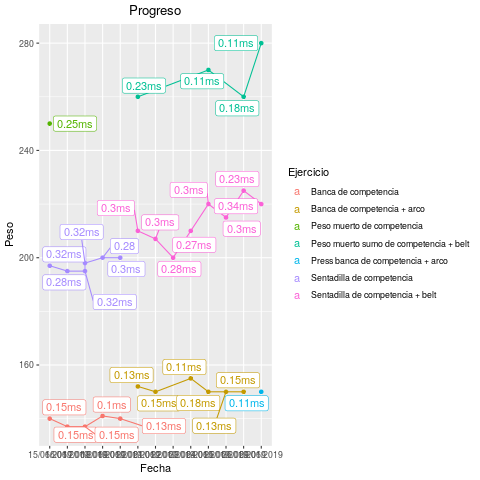
\includegraphics[width=.9\linewidth]{tmp.png}
\end{center}
\end{document}
